\documentclass[a4paper]{article}

\usepackage[english]{babel}
\usepackage[utf8]{inputenc}
\usepackage{amsmath}
\usepackage{graphicx}
\usepackage{subfigure}

\usepackage[colorinlistoftodos]{todonotes}
% 导入包
\usepackage{hyperref}
% 格式设置
\hypersetup{hidelinks,
	colorlinks=true,
	allcolors=black,
	pdfstartview=Fit,
	breaklinks=true}
	
\title{EDA234 Lab 1 - Reflection:  Lab Tutorial}

\author{Weihan Gao weihanga@chalmers.se} 

\date{\today}

\begin{document}
\sloppy
\maketitle


\section{Introduction}
\label{sec:introduction}
We created the second counter and show them on the two digital 7-segments. But the registers we used are 53. 

\centering
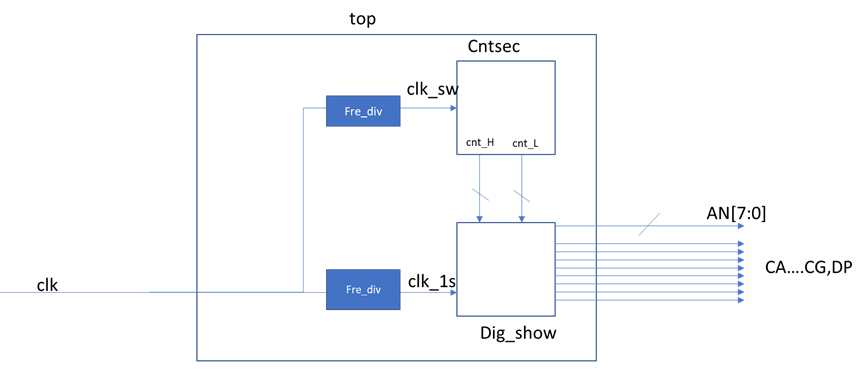
\includegraphics[width=1\textwidth]{1.png}
\caption{\label{fig:data}Registers utilization}
\end{figure}



\section{Second hand in}
We

\newpage


\begin{figure}[h]
\centering
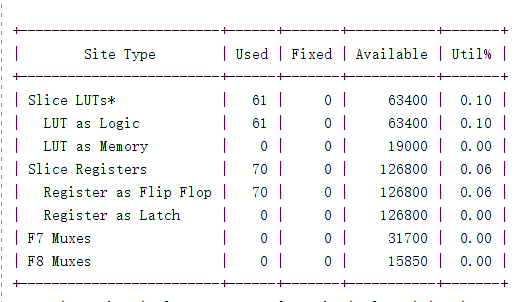
\includegraphics[width=1\textwidth]{2.png}
\caption{\label{fig:data}Coefficient array and Timetable of input x.}
\end{figure}



\caption{Timing summary.}
\end{figure}
%\begin{figure}[h]
%\centering
%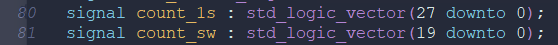
\includegraphics[width=1\textwidth]{5.png}
%\caption{\label{fig:data}.}
%\end{figure}
%
%\begin{figure}[h]
%\centering
%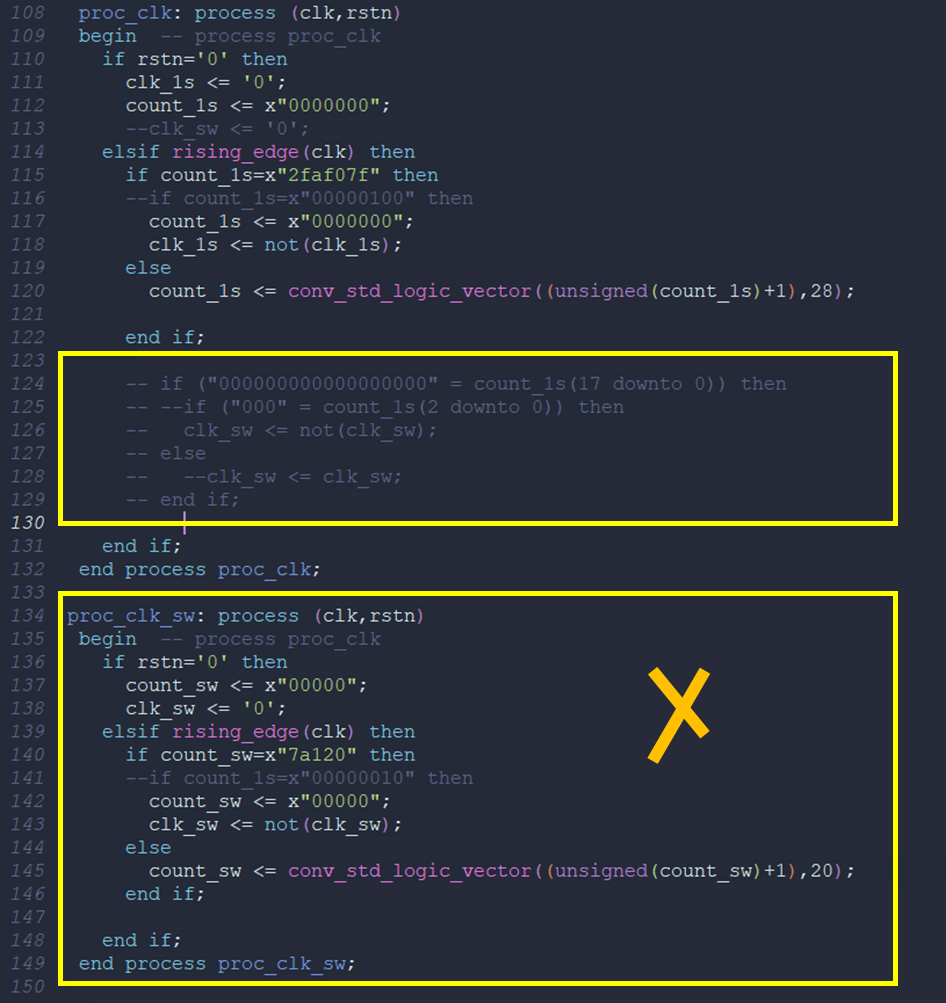
\includegraphics[width=1\textwidth]{6.png}
%\caption{\label{fig:data}.}
%\end{figure}


\newpage



\subsection{Project Summary}
Apart from the Settings, Board Part, the Project Summary contains Synthesis and Implementation message, timing message, the Resource Utilization in post-synthesis and post-implementation, DRC report, and the power consumed. When we map the RTL designs in an FPGA board, we need to consider the timing, and resource usage after correcting all critical warnings in Synthesis and Implementation, also need to choose the correct aim FPGA board.
\begin{figure}[h]
%\centering
\subfigure[Synthesis and DRC]
{
    \begin{minipage}[b]{.5\linewidth}
        %\centering
        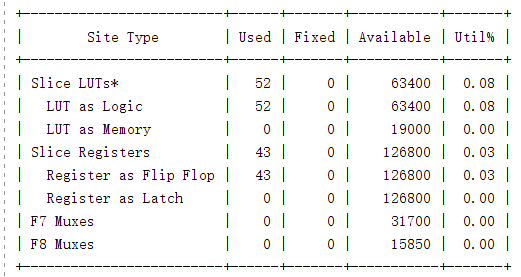
\includegraphics[width=5.5cm,height=4.cm]{7.png}
    \end{minipage}
}
\subfigure[Implementation and Timing]
{
 	\begin{minipage}[b]{.5\linewidth}
        %\centering
        \includegraphics[width=5.5cm,height=4.cm]{8.png}
    \end{minipage}
}

\caption{Project Summary.}
\end{figure}





























\iffalse
\section{Experiment 1-2 pages}
\subsection{Fabrication}
Explain a step-by-step recipe for fabrication here. How long did you etch and why? What is an Ohmic contact?
\subsection{Experimental set-up}
Explain the experimental set-up here. Use a schematic picture (make it yourself in photoshop, paint, ...) to show how the components are connected. Briefly explain how a lock-in amplifier works.

\section{Results and interpretation 2-3 pages}
Show a graph of the longitudinal resistivity ($\rho_{xx}$) and Hall resistivity ($\rho_{xy}$) versus magnetic field, extracted from the raw data shown in figure \ref{fig:data}. You will have the link to the data in your absalon messages, if not e-mail Guen (guen@nbi.dk). Explain how you calculated these values, and refer to the theory.

\begin{figure}
\centering
\includegraphics[width=1\textwidth]{raw_data.png}
\caption{\label{fig:data}Raw (unprocessed) data. Replace this figure with the one you've made, that shows the resistivity.}
\end{figure}

\subsection{Classical regime}
Calculate the sheet electron density $n_{s}$ and electron mobility $\mu$ from the data in the low-field regime, and refer to the theory in section \ref{sec:theory}. Explain how you retrieved the values from the data (did you use a linear fit?).
Round values off to 1 or 2 significant digits: 8.1643 ~= 8.2. Also, 5e-6 is easier to read than 0.000005.

!OBS: This part is optional (only if you have time left).
Calculate the uncertainty as follows: \newline $u(f(x, y, z)) = \sqrt{(\frac{\delta f}{\delta{x}} u(x))^{2} + (\frac{\delta f}{\delta{y}} u(y))^{2} + (\frac{\delta f}{\delta{z}} u(z))^{2}}$, where $f$ is the calculated value ($n_{s}$ or $\mu$), $x, y, z$ are the variables taken from the measurement and $u(x)$ is the uncertainty in x (and so on).

\subsection{Quantum regime}
Calculate $n_{s}$ for the high-field regime.
Show a graph of the longitudinal conductivity ($\rho_{xx}$) and Hall conductivity($\rho_{xy}$) \textbf{in units of the resistance quantum} ($\frac{h}{e^{2}}$), depicting the integer filling factors for each plateau.
Show a graph of the plateau number versus its corresponding value of $1/B$. From this you can determine the slope, which you use to calculate the electron density.
Again, calculate the uncertainty for your obtained values.

\section{Discussion 1/2-1 page}
Discuss your results. Compare the two values of $n_{s}$ that you've found in the previous section. Compare your results with literature and comment on the difference. If you didn't know the value of the resistance quantum, would you be able to deduce it from your measurements? If yes/no, why?

\newpage
\section{Some LaTeX tips}
\label{sec:latex}
\subsection{How to Include Figures}

First you have to upload the image file (JPEG, PNG or PDF) from your computer to writeLaTeX using the upload link the project menu. Then use the includegraphics command to include it in your document. Use the figure environment and the caption command to add a number and a caption to your figure. See the code for Figure \ref{fig:frog} in this section for an example.

\begin{figure}
\centering
\includegraphics[width=0.3\textwidth]{frog.jpg}
\caption{\label{fig:frog}This frog was uploaded to writeLaTeX via the project menu.}
\end{figure}

\subsection{How to Make Tables}

Use the table and tabular commands for basic tables --- see Table~\ref{tab:widgets}, for example.

\begin{table}
\centering
\begin{tabular}{l|r}
Item & Quantity \\\hline
Widgets & 42 \\
Gadgets & 13
\end{tabular}
\caption{\label{tab:widgets}An example table.}
\end{table}

\subsection{How to Write Mathematics}

\LaTeX{} is great at typesetting mathematics. Let $X_1, X_2, \ldots, X_n$ be a sequence of independent and identically distributed random variables with $\text{E}[X_i] = \mu$ and $\text{Var}[X_i] = \sigma^2 < \infty$, and let

\begin{equation}
S_n = \frac{X_1 + X_2 + \cdots + X_n}{n}
      = \frac{1}{n}\sum_{i}^{n} X_i
\label{eq:sn}
\end{equation}

denote their mean. Then as $n$ approaches infinity, the random variables $\sqrt{n}(S_n - \mu)$ converge in distribution to a normal $\mathcal{N}(0, \sigma^2)$.

The equation \ref{eq:sn} is very nice.

\subsection{How to Make Sections and Subsections}

Use section and subsection commands to organize your document. \LaTeX{} handles all the formatting and numbering automatically. Use ref and label commands for cross-references.

\subsection{How to Make Lists}

You can make lists with automatic numbering \dots

\begin{enumerate}
\item Like this,
\item and like this.
\end{enumerate}
\dots or bullet points \dots
\begin{itemize}
\item Like this,
\item and like this.
\end{itemize}
\dots or with words and descriptions \dots
\begin{description}
\item[Word] Definition
\item[Concept] Explanation
\item[Idea] Text
\end{description}

We hope you find write\LaTeX\ useful, and please let us know if you have any feedback using the help menu above.

\begin{thebibliography}{9}
\bibitem{nano3}
  K. Grove-Rasmussen og Jesper Nygård,
  \emph{Kvantefænomener i Nanosystemer}.
  Niels Bohr Institute \& Nano-Science Center, Københavns Universitet

\end{thebibliography}
\fi



\end{document}